\section{Faza II — turniej główny}
\label{sec:phase2}

W fazie II sześciu reprezentantów wyłonionych w fazie I rywalizowało między sobą w pełnym turnieju round-robin. Celem było sprawdzenie, które warianty agenta są najskuteczniejsze i w jakim stopniu.

\subsection{Wyniki ogólne}

Faza II sprawdza, które z zaproponowanych modyfikacji rzeczywiście poprawiają skuteczność agenta i o ile. Tabela~\ref{tab:phase2-aggregate-results} zestawia wyniki zbiorcze wszystkich sześciu reprezentantów w turnieju round-robin (\(90\,000\) partii na agenta). Najwyższą skuteczność osiągnął wariant \textit{21 głębokościowy} (\(61{,}03\%\) zwycięstw), drugie miejsce zajął wariant \textit{28 parametrów} (\(50{,}55\%\)). Pozostałe konfiguracje mieszczą się w przedziale \(46\%\)--\(48\%\), co oznacza, że różnice między nimi są wyraźnie mniejsze niż dystans do zwycięzcy.

\begin{table}[ht]
\centering
\small
\begin{tabular}{lrrr}
\toprule
Wariant & Wygrane & Partie & Wskaźnik zwycięstw [\%] \\
\midrule
\textit{21 głębokościowy} & 54923 & 90000 & 61,03 \\
\textit{28 parametrów} & 45495 & 90000 & 50,55 \\
\textit{63 płynny} & 43036 & 90000 & 47,82 \\
\textit{28 znormalizowany} & 42953 & 90000 & 47,73 \\
\textit{bazowy 21} & 41878 & 90000 & 46,53 \\
\textit{63 parametry} & 41715 & 90000 & 46,35 \\
\bottomrule
\end{tabular}
\caption{Wyniki zbiorcze turnieju głównego fazy II.}
\label{tab:phase2-aggregate-results}
\end{table}


\definecolor{wrLow}{RGB}{178,24,43}
\definecolor{wrMid}{RGB}{247,247,247}
\definecolor{wrHigh}{RGB}{33,102,172}

\begin{table}[ht]
\centering
\scriptsize
\setlength{\tabcolsep}{3pt}
\caption{Macierz wskaźnika zwycięstw agent vs agent w turnieju fazy II (wiersze: oceniany agent, kolumny: przeciwnik).}
\label{tab:phase2-agent-vs-agent-heatmap}
\begin{tabular}{lrrrrrr}
\toprule
Agent & \rotatebox{60}{\textit{bazowy 21}} & \rotatebox{60}{\textit{63 parametry}} & \rotatebox{60}{\textit{63 płynny}} & \rotatebox{60}{\textit{28 parametrów}} & \rotatebox{60}{\textit{28 znormalizowany}} & \rotatebox{60}{\textit{21 głębokościowy}} \\
\midrule
\textit{bazowy 21} & \cellcolor{black!8}-- & \cellcolor{wrHigh!1}50,2 & \cellcolor{wrLow!5}48,6 & \cellcolor{wrLow!14}46,5 & \cellcolor{wrLow!4}49,0 & \cellcolor{wrLow!47}38,3 \\
\textit{63 parametry} & \cellcolor{wrLow!1}49,9 & \cellcolor{black!8}-- & \cellcolor{wrLow!6}48,5 & \cellcolor{wrLow!14}46,5 & \cellcolor{wrLow!4}49,1 & \cellcolor{wrLow!48}37,9 \\
\textit{63 płynny} & \cellcolor{wrHigh!5}51,4 & \cellcolor{wrHigh!6}51,6 & \cellcolor{black!8}-- & \cellcolor{wrLow!9}47,7 & \cellcolor{wrLow!2}49,6 & \cellcolor{wrLow!44}38,9 \\
\textit{28 parametrów} & \cellcolor{wrHigh!14}53,5 & \cellcolor{wrHigh!14}53,5 & \cellcolor{wrHigh!9}52,3 & \cellcolor{black!8}-- & \cellcolor{wrHigh!10}52,6 & \cellcolor{wrLow!37}40,8 \\
\textit{28 znormalizowany} & \cellcolor{wrHigh!4}51,0 & \cellcolor{wrHigh!4}50,9 & \cellcolor{wrHigh!2}50,4 & \cellcolor{wrLow!10}47,4 & \cellcolor{black!8}-- & \cellcolor{wrLow!44}38,9 \\
\textit{21 głębokościowy} & \cellcolor{wrHigh!47}61,7 & \cellcolor{wrHigh!48}62,1 & \cellcolor{wrHigh!44}61,1 & \cellcolor{wrHigh!37}59,2 & \cellcolor{wrHigh!44}61,1 & \cellcolor{black!8}-- \\
\bottomrule
\end{tabular}
\end{table}


Tabela~\ref{tab:phase2-agent-vs-agent-heatmap} potwierdza i uzupełnia wyniki zbiorcze. Wariant \textit{21 głębokościowy} wygrał z każdym rywalem w przedziale \(59{,}2\%\)--\(62{,}1\%\), co oznacza, że przewaga ma charakter globalny i nie jest ograniczona do jednego rywala. Najtrudniejszym przeciwnikiem dla wariantu \textit{21 głębokościowego} okazał się \textit{28 parametrów} --- jedyny wariant, który zdołał utrzymać wynik powyżej \(40\%\) w bezpośrednim starciu. Pozostałe cztery warianty często oscylują wokół \(50\%\) między sobą, co oznacza, że różnice w ich rankingu zbiorczym wynikają bardziej z sumy małych przewag niż z wyraźnej dominacji w konkretnych starciach. Wyjątkiem jest para \textit{28 parametrów} vs \textit{28 znormalizowany}: tu przewaga pierwszego (\(52{,}6\%\)) jest wyraźniejsza niż w pozostałych zestawieniach tej grupy.

Wniosek ogólny, jaki płynie z tej części pracy, to że największą poprawę jakości zapewnia nie dalsze zwiększanie liczby współczynników, lecz zmiana procesu podejmowania decyzji. Przy danym budżecie obliczeniowym większy zysk przynosi lepsza metoda planowania akcji niż dodawanie kolejnych cech oceny.

Faza II potwierdza też praktyczny sukces całego podejścia badawczego: zaproponowane modyfikacje --- z wyjątkiem wariantu \textit{63 parametry} --- przewyższają wariant bazowy. Najlepszy wariant ma wyraźną przewagę nad każdym rywalem. Pokazuje to, że zaproponowane rozszerzenia naprawdę poprawiają skuteczność agenta, a nie są tylko formalnymi zmianami.

\subsection{Wpływ normalizacji (28 vs 28 znormalizowany)}

Bezpośrednie porównanie \(28\) vs \(28\) znormalizowany wskazuje na przewagę wariantu bez normalizacji (\(\approx 52{,}6\%\) w bezpośrednim starciu). Oba warianty mają podobny poziom względem części pozostałych agentów, co sugeruje, że normalizacja nie powoduje zasadniczej zmiany w sposobie gry agenta, ale jedynie obniża jego skuteczność.

\begin{figure}[ht]
\centering
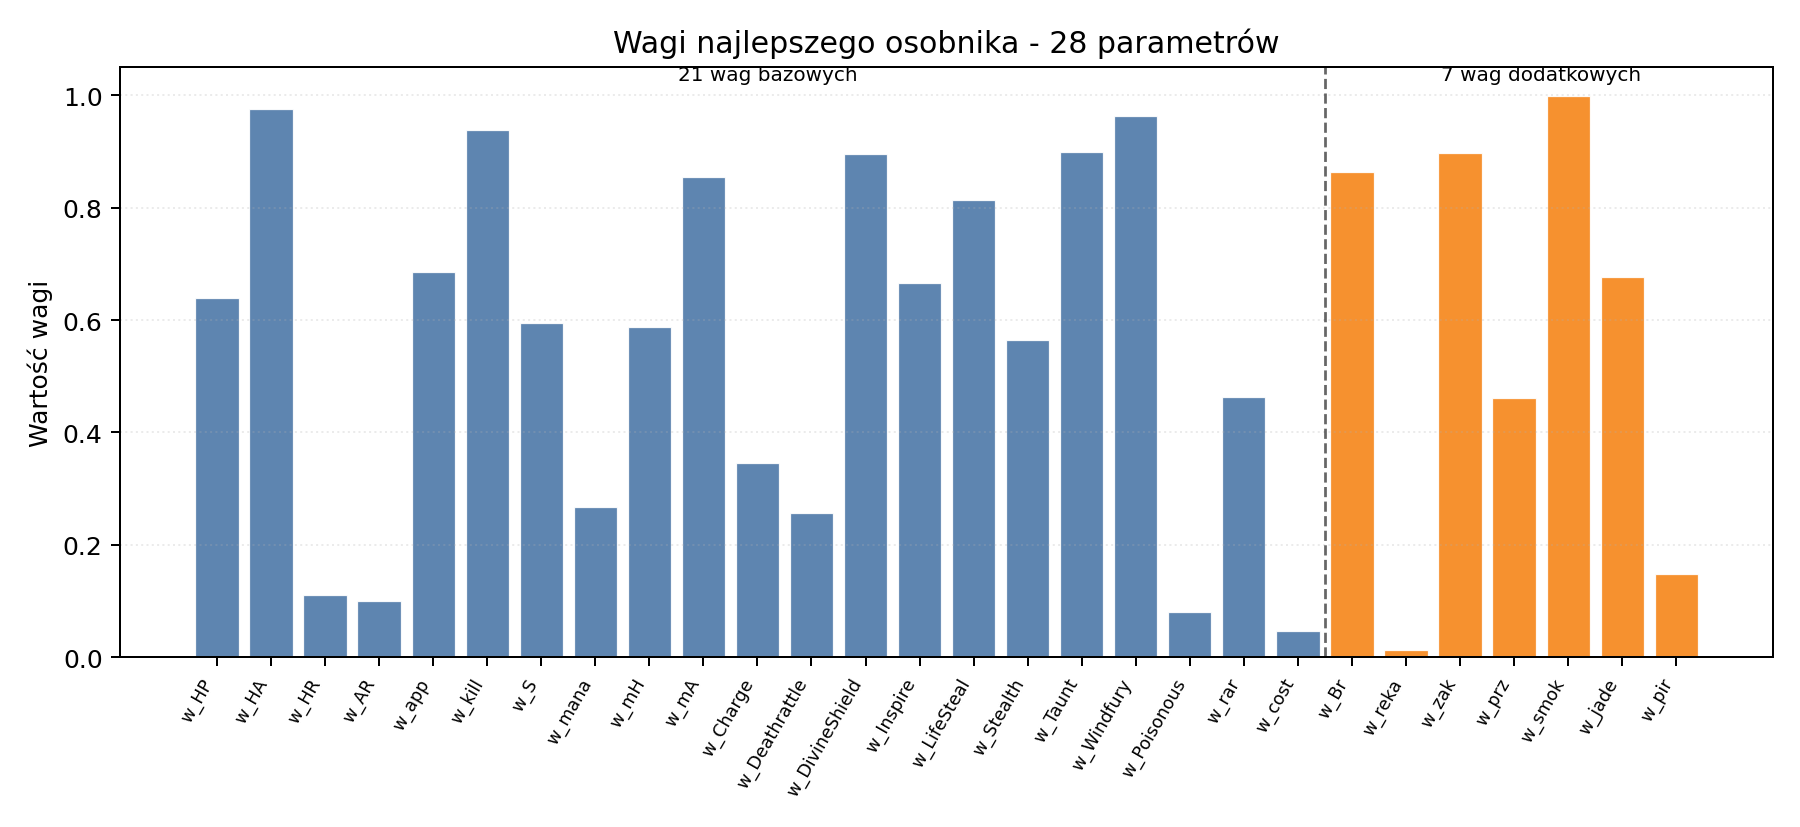
\includegraphics[width=0.95\textwidth]{chapters/07analysis/generated/figures/weights_best_v28.png}
\caption{Wykres wag reprezentanta wariantu 28-parametrowego. Pierwsze 21 wag odpowiada cechom bazowym, ostatnie 7 wag to cechy dodatkowe.}
\label{fig:weights-v28}
\end{figure}

\begin{figure}[ht]
\centering
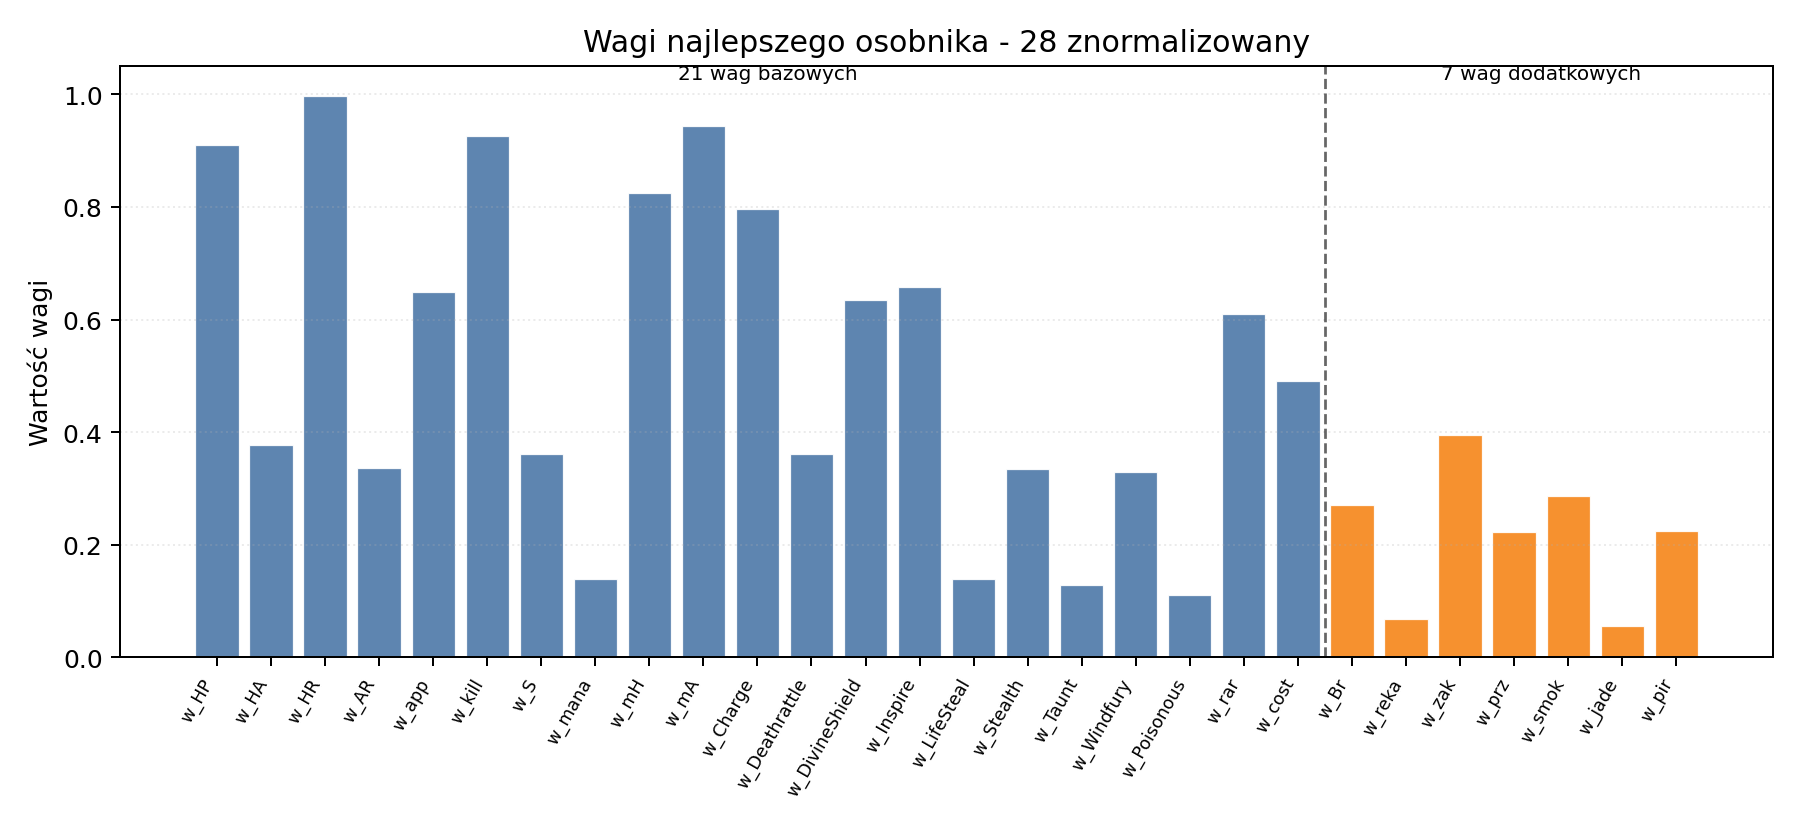
\includegraphics[width=0.95\textwidth]{chapters/07analysis/generated/figures/weights_best_v28norm.png}
\caption{Wykres wag reprezentanta wariantu 28-parametrowego z normalizacją.}
\label{fig:weights-v28norm}
\end{figure}

Rysunki~\ref{fig:weights-v28} i~\ref{fig:weights-v28norm} pokazują, że różnica nie wynika z jednej wagi, lecz z całego rozkładu między częścią bazową a nowymi siedmioma cechami. W wariancie bez normalizacji część nowych wag ma większe amplitudy, co wzmacnia ich wpływ w sytuacjach, dla których zostały zaprojektowane. W wariancie z normalizacją więcej wag jest bliżej środka skali, więc podejście agenta jest bardziej zachowawcze i mniej selektywne.

Normalizacja stabilizuje zachowanie modelu, ale może osłabiać cechy, które w niektórych sytuacjach powinny działać wyraźniej. Wariant z normalizacją zyskuje regularność, ale może tracić część zdolności do silnej reakcji w trudnych stanach gry.

Jedną z prawdopodobnych przyczyn słabszego wyniku wariantu \textit{28 znormalizowany} może być sama metoda wyznaczania maksymalnych progów parametrów. W badaniu pułap dla każdej cechy wyznaczano na podstawie wartości maksymalnej obserwowanej po rozegraniu $\approx1.08$ miliona gier Taki sposób jest wrażliwy na rzadkie anomalie. Pojedynczy, bardzo wysoki odczyt może zawyżyć pułap i w konsekwencji niesprawiedliwie zaniżyć znormalizowane wartości tej wagi. W kolejnych eksperymentach warto rozważyć bardziej odporne podejście, np.\ użycie mediany lub średniej z \(N\) najwyższych obserwacji i obcięcie wartości powyżej tego progu do \(1\).

Najistotniejsze okazały się następujące cechy: \textit{Br}, \textit{Zak}, \textit{Smok} i \textit{Jade}. Te parametry niosą ze sobą jasną informację o planie tury. \textit{Br} zwykle przekłada się na tempo wymian i kontrolę stołu. \textit{Zak} zwiększa wartość sekwencji z zaklęciami, więc pomaga wybierać bardziej opłacalne układy ruchów. \textit{Smok} i \textit{Jade} wzmacniają decyzje związane z synergią talii i planem na kilka tur do przodu.

Mniejsza rola \textit{Prz} i \textit{Pir} wynika z sytuacyjności tych cech --- dają zysk głównie w części układów stołu i części zestawień talii, więc w ujęciu globalnym mają mniejszy wpływ niż cechy, które działają często i szeroko. Z tego powodu model traktuje je jako dodatek, a niekoniecznie jako główny trzon decyzji.

Bardzo mała rola \textit{Ręka} jest spójna z praktyką gry w tym ustawieniu eksperymentu. W tym zbiorze talii i przy tym stylu oceny większy wpływ ma bieżący stan stołu, tempo rozgrywki i aktywne synergie niż sama liczba kart na ręce. Model premiuje dobrą sytuację na planszy niż zapas kart, dlatego waga \textit{Ręka} spada blisko zera.

\paragraph{Wniosek z porównania agentów z 28 parametrami}
Przejście z 21 do 28 cech poprawia skuteczność agenta w obu wersjach: wariant \textit{28 parametrów} wygrał z agentem bazowym w bezpośrednim starciu wynikiem \(53{,}5\%\), a \textit{28 znormalizowany} --- \(51{,}0\%\). Wybór sposobu skalowania cech ma jednak znaczenie. Wariant bez normalizacji wyprzedza agenta znormalizowanego o \(\approx 2{,}5\)p.p. w rywalizacji przeciw agentowi bazowemu, a w bezpośrednim starciu uzyskał \(52{,}6\%\) odsetka zwycięstw. Odpowiedź na pytanie badawcze nr 1 (RQ1) jest więc pozytywna: rozszerzenie przestrzeni cech z 21 do 28 poprawia jakość agenta, ale pełny potencjał tej modyfikacji ujawnia się tylko bez nadmiernego wygładzania wartości cech.

\subsection{Wpływ podziału fazowego (63 vs 63 płynny)}

W parze \(63\) vs \(63\) płynny, wariant płynny ma lekką przewagę --- w bezpośrednim starci odsetek zwycięstw wynosi \(51{,}6\%\). Jest to ciekawy wynik, ponieważ oba warianty mają tyle samo parametrów, a różni je tylko sposób dekodowania wag i przenoszenia ich między fazami gry.

\begin{figure}[ht]
\centering
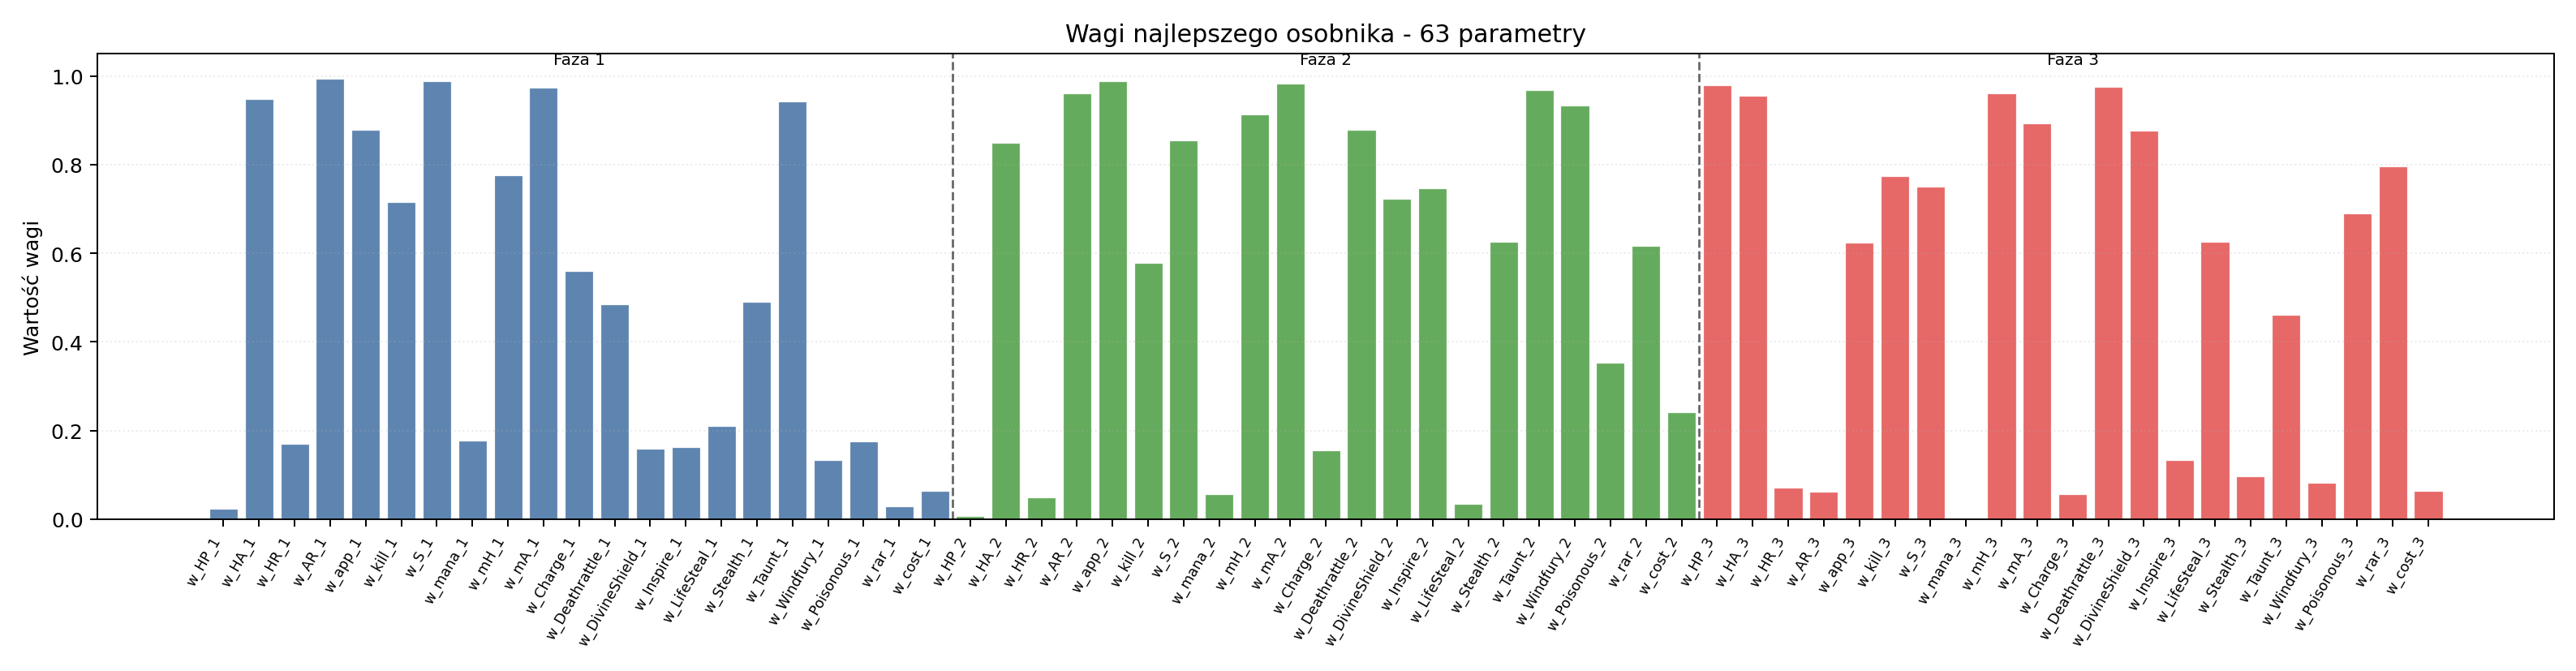
\includegraphics[width=0.98\textwidth]{chapters/07analysis/generated/figures/weights_best_v63.png}
\caption{Wykres wag reprezentanta wariantu \textit{63-parametrowego} z niezależnymi fazami.}
\label{fig:weights-v63}
\end{figure}

\begin{figure}[ht]
\centering
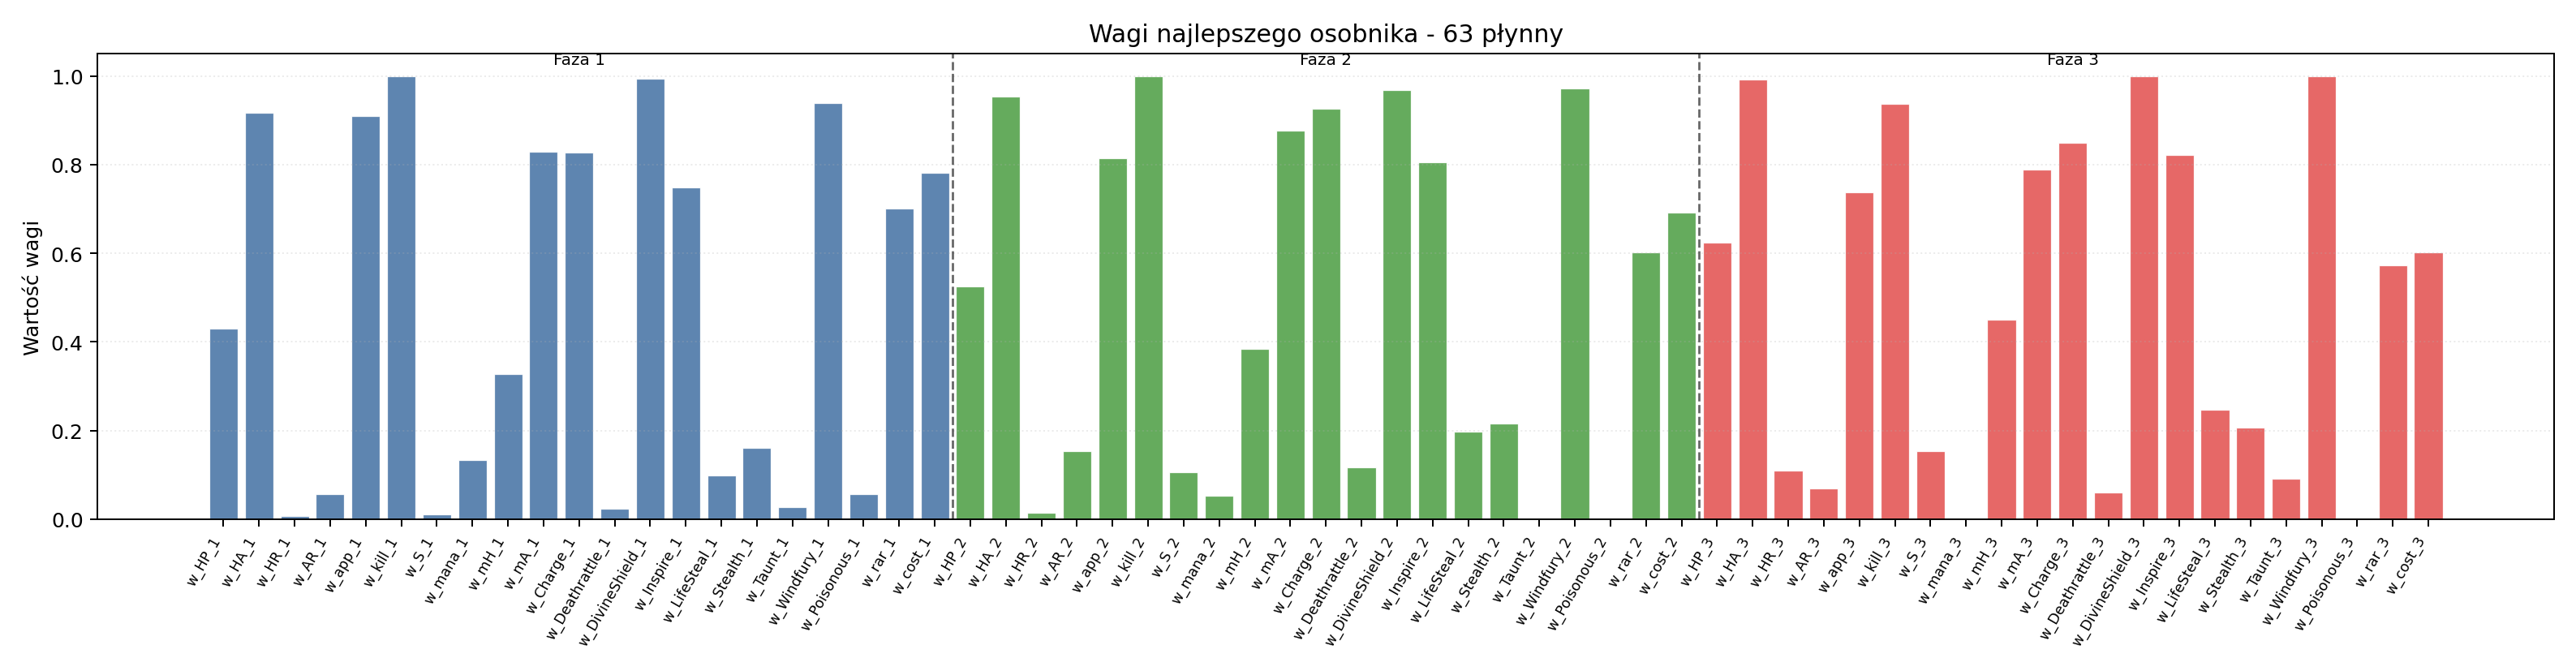
\includegraphics[width=0.98\textwidth]{chapters/07analysis/generated/figures/weights_best_v63smooth.png}
\caption{Wykres wag reprezentanta wariantu \textit{63-parametrowego} z płynnym przejściem faz (wagi po dekodowaniu i ograniczeniu do przedziału \([0,1]\)).}
\label{fig:weights-v63smooth}
\end{figure}

Rysunki~\ref{fig:weights-v63} i~\ref{fig:weights-v63smooth} pokazują, że wariant płynny ogranicza gwałtowne skoki między fazą 1, 2 i 3. Wynika to z implementacji, w której wagi kolejnych faz powstają przez przesunięcia w kontrolowanym zakresie i są ograniczane do dopuszczalnego przedziału. W praktyce zmniejsza to ryzyko niestabilnych przełączeń strategii przy zmianie fazy rozgrywki.

Wariant 63-parametrowy bez wygładzania daje większą swobodę niezależnego strojenia każdej fazy, ale łatwiej w nim o niespójne podejście decyzyjne. Wariant płynny ogranicza te swobodę, ale zwiększa spójność zachowania, co praktycznie przekłada się na niewielką, ale powtarzalną przewagę.

\paragraph{Wniosek z porównania agentów z 63 parametrami}
Reprezentacja fazowa jest użyteczna, ale jej skuteczność zależy od mechanizmu łączenia faz. Wariant \textit{63 płynny} wygrał z agentem bazowym wynikiem \(51{,}4\%\) w bezpośrednim starciu, podczas gdy \textit{63 parametry} bez wygładzania przegrał z wariantem bazowym (\(49{,}9\%\)). Bezpośrednie starcie między wariantami 63-parametrowymi daje wynik \(51{,}6\%\) zwycięstw na korzyść wariantu płynnego. Odpowiedź na pytanie badawcze nr 2 (RQ2) jest pozytywna pod pewnym warunkiem: sam wzrost liczby parametrów nie poprawia jakości agenta --- potrzebny jest mechanizm zapewniający spójność decyzji między fazami gry.

\subsection{Wpływ podejścia głębokościowego (bazowy 21 vs 21 głębokościowy)}

Największy efekt w całej fazie II widać w porównaniu \textit{bazowy 21} vs \textit{21 głębokościowy}: wariant głębokościowy osiąga około \(61{,}7\%\) zwycięstw w bezpośrednim starciu. Co ważne, ta skala przewagi utrzymuje się również wobec pozostałych wariantów --- nie jest więc wynikiem jednego sprzyjającego zestawienia.

\begin{figure}[ht]
\centering
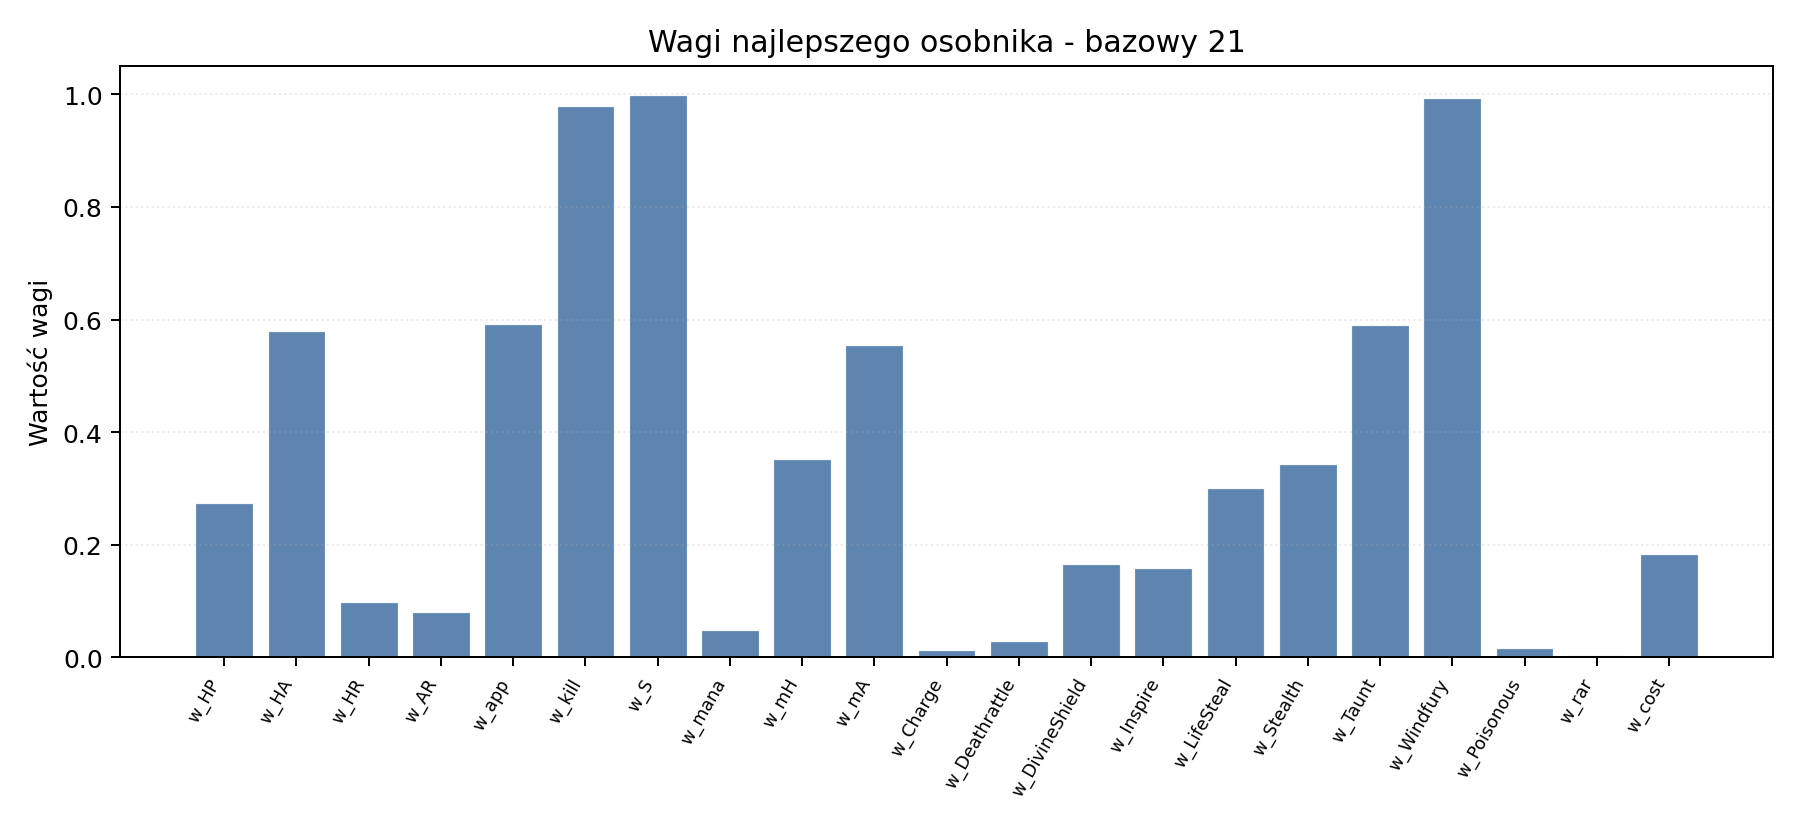
\includegraphics[width=0.95\textwidth]{chapters/07analysis/generated/figures/weights_best_base21.png}
\caption{Wykres wag reprezentanta wariantu \textit{bazowego 21-parametrowego}.}
\label{fig:weights-base21}
\end{figure}

\begin{figure}[ht]
\centering
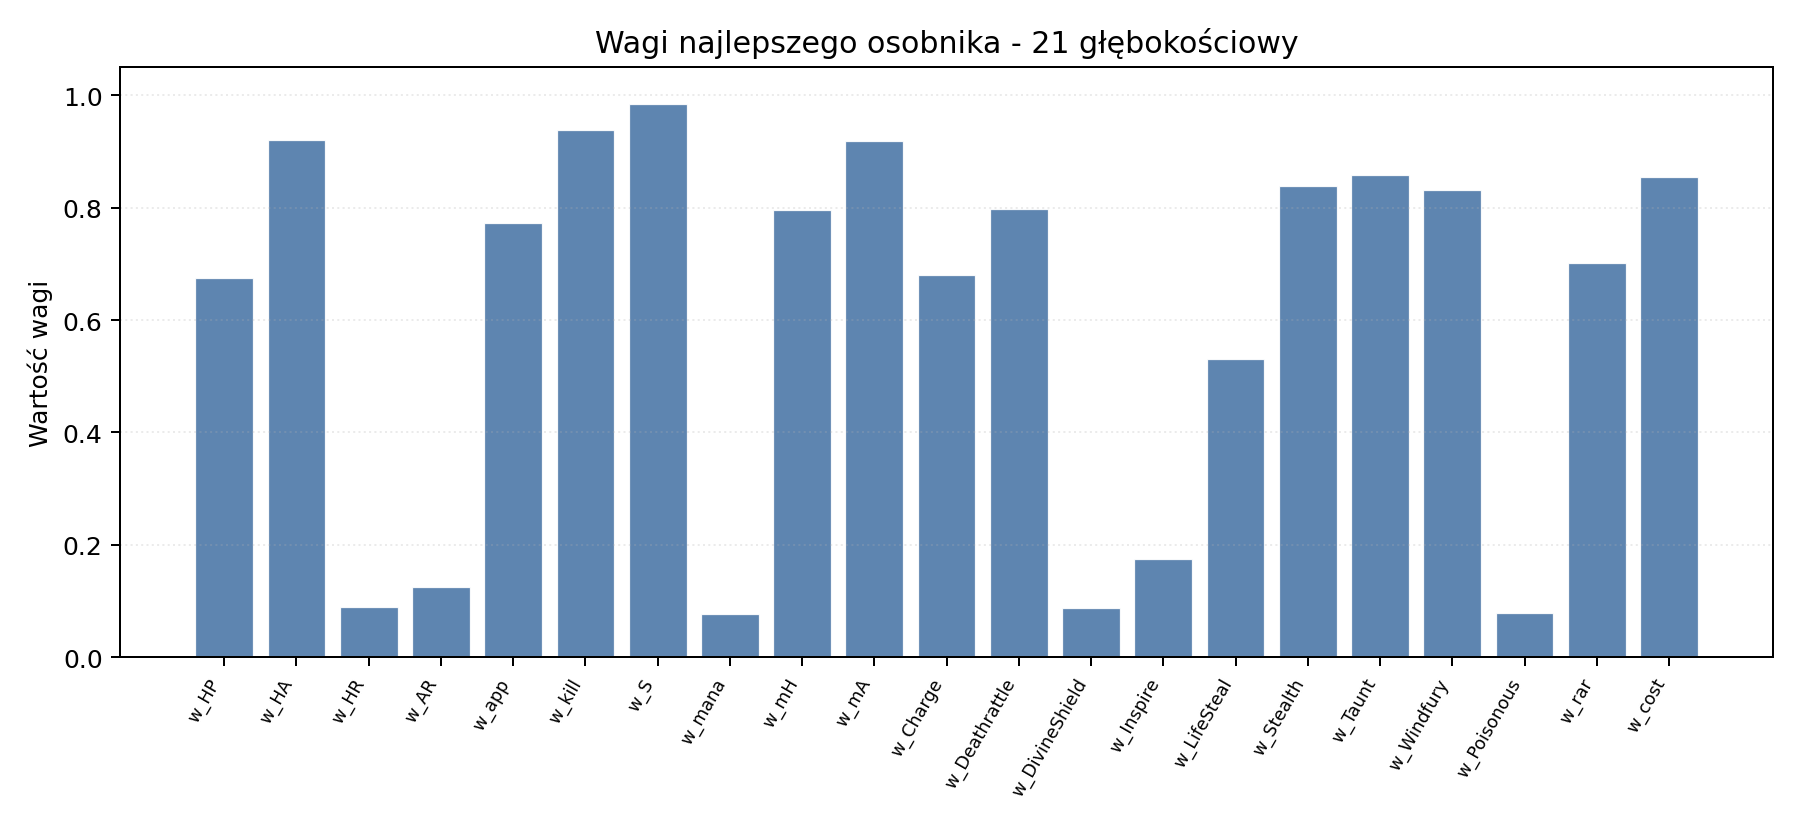
\includegraphics[width=0.95\textwidth]{chapters/07analysis/generated/figures/weights_best_v21depth.png}
\caption{Wykres wag reprezentanta wariantu \textit{21-parametrowego} z przeszukiwaniem głębokościowym.}
\label{fig:weights-v21depth}
\end{figure}

Porównanie rysunków~\ref{fig:weights-base21} i~\ref{fig:weights-v21depth} pokazuje, że sama zmiana wag nie wyjaśnia całkowicie różnicy w jakości. Wariant głębokościowy zmienia przede wszystkim kontekst, w którym wagi są używane. Ocena stanu planszy jest osadzona w procesie planowania sekwencji akcji, a nie jedynie w podejmowaniu najlepszej decyzji tu i teraz. Dzięki temu agent częściej wybiera ruchy korzystne w perspektywie kilku kroków, nawet jeśli pojedynczo nie wydają się optymalne.

W praktyce oznacza to wyraźną przewagę w sytuacjach, gdzie korzyść natychmiastowa stoi w konflikcie z przygotowaniem kolejnej tury. Wariant bazowy częściej wybiera ruch lokalnie dobry, natomiast wariant głębokościowy częściej wybiera sekwencję prowadzącą do lepszej pozycji końcowej.

\paragraph{Wniosek z porównania agenta bazowego z głębokościowym.}
Dodanie przeszukiwania głębokościowego daje największy i najbardziej stabilny zysk jakościowy spośród wszystkich badanych modyfikacji. Wariant \textit{21 głębokościowy} wygrał z agentem bazowym wynikiem \(61{,}7\%\) w bezpośrednim starciu i utrzymał przewagę powyżej \(59\%\) przeciwko każdemu z pozostałych wariantów. Odpowiedź na pytanie badawcze nr 3 (RQ3) jest więc jednoznaczna i zdecydowanie pozytywna: zmiana sposobu podejmowania decyzji przynosi większy zysk niż jakiekolwiek rozszerzenie przestrzeni parametrów funkcji oceny.

\subsection{Struktura wag reprezentantów fazy II}

\begin{figure}[ht]
\centering
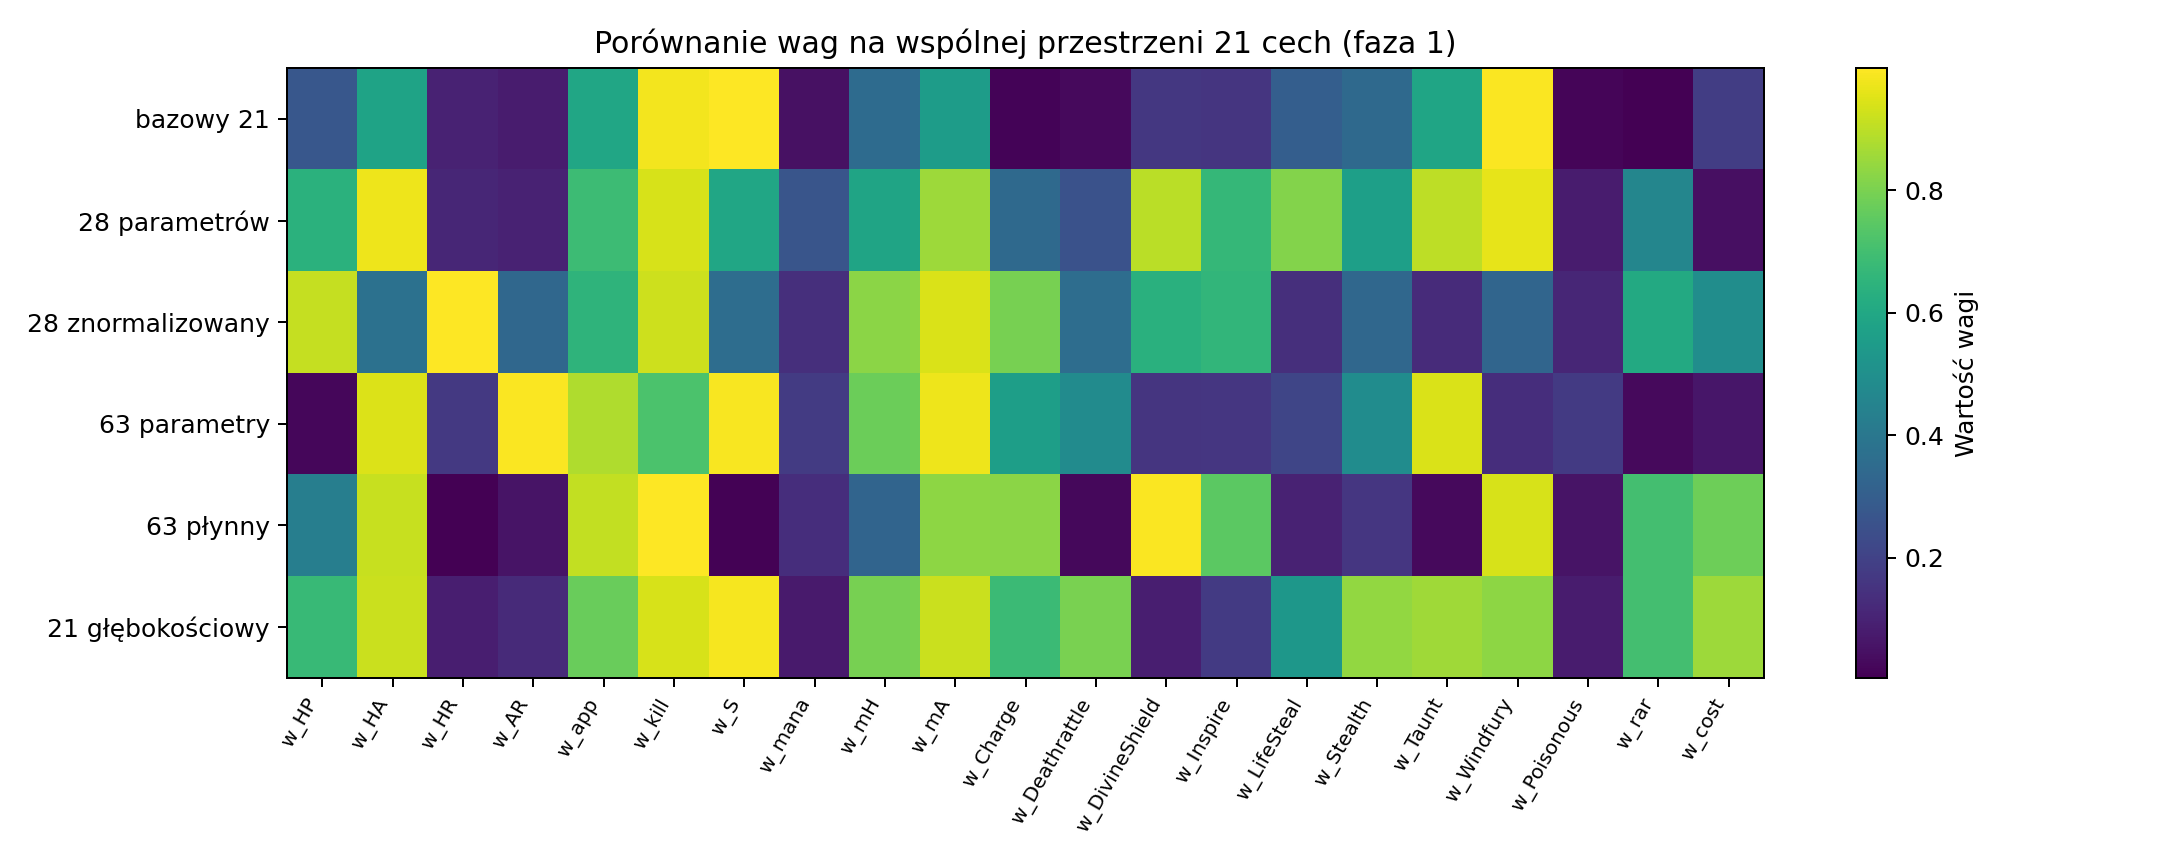
\includegraphics[width=0.90\textwidth]{chapters/07analysis/generated/figures/weights_heatmap_base21.png}
\caption{Porównanie wag reprezentantów fazy II we wspólnej przestrzeni 21 cech bazowych.}
\label{fig:weights-heatmap-base21}
\end{figure}

Rysunek~\ref{fig:weights-heatmap-base21} zestawia zwycięskie konfiguracje wag po sprowadzeniu ich do tego samego układu 21 cech. Dla wariantów 21-parametrowych porównano pełny wektor wag, a dla wariantów 28-parametrowych i 63-parametrowych --- pierwsze 21 wag z wektora.

Na mapie cieplnej widać, że większość wariantów ma zbliżony układ wielu wag --- część współczynników wygląda podobnie między agentami, a różnice dotyczą głównie tego, jak mocno dana waga jest zwiększona lub obniżona. Wariant \textit{21 głębokościowy} częściej ma inny rozkład wartości niż pozostałe, ale nie jest całkowicie odseparowany od reszty grupy. Najprostszy wniosek z tego rysunku jest taki, że jego przewaga z fazy II nie wygląda na efekt jednej wyjątkowej wagi, lecz raczej na efekt całego układu współczynników i sposobu podejmowania decyzji.

\subsection{Podsumowanie fazy II}

Wynik turnieju głównego prowadzi do trzech wniosków. Po pierwsze, większa liczba parametrów nie oznacza automatycznie lepszego agenta: przejście \(21 \rightarrow 28\) daje największy zysk wśród modyfikacji reprezentacji — wariant \textit{28 parametrów} zajął drugie miejsce w turnieju, uzyskując \(50{,}55\%\) zwycięstw i wyraźnie przewyższa wariant bazowy w bezpośrednich starciach. Dalsze przejście \(28 \rightarrow 63\) nie powtarza tego efektu: zysk jest niewielki i zależy od implementacji mechanizmu łączenia faz. Po drugie, największą przewagę w całym turnieju uzyskał wariant \textit{21 głębokościowy} (tabela~\ref{tab:phase2-aggregate-results}), co wskazuje, że ważniejsza od samej liczby wag jest zmiana sposobu podejmowania decyzji. Po trzecie, cztery z pięciu pozostałych wariantów osiągnęły wyższy odsetek zwycięstw niż agent bazowy. Jedynie wariant \textit{63 parametry} pozostał na podobnym poziomie — agent bazowy wygrał, uzyskując \(50{,}2\%\) zwycięstw w bezpośrednim starciu.

Odpowiedzi na pytania RQ1--RQ3 są pozytywne, ale efekty różnią się w skali: rozszerzenie cech \(21 \rightarrow 28\) (RQ1) daje wyraźny zysk, reprezentacja fazowa \(28 \rightarrow 63\) (RQ2) poprawia wyniki tylko przy odpowiednim mechanizmie łączenia faz, natomiast podejście głębokościowe (RQ3) przynosi zdecydowanie największą poprawę spośród wszystkich badanych modyfikacji.
